\documentclass[letterpaper]{article}

% if you need to pass options to natbib, use, e.g.:
%     \PassOptionsToPackage{numbers, compress}{natbib}
% before loading neurips_2018

% ready for submission
% \usepackage{neurips_2018}

% to compile a preprint version, e.g., for submission to arXiv, add add the
% [preprint] option:
%     \usepackage[preprint]{neurips_2018}

% to compile a camera-ready version, add the [final] option, e.g.:
     \usepackage[final]{neurips_2018}

% to avoid loading the natbib package, add option nonatbib:
%     \usepackage[nonatbib]{neurips_2018}

\usepackage[utf8]{inputenc} % allow utf-8 input
\usepackage[T1]{fontenc}    % use 8-bit T1 fonts
\usepackage{hyperref}       % hyperlinks
\usepackage{url}            % simple URL typesetting
\usepackage{booktabs}       % professional-quality tables
\usepackage{amsfonts}       % blackboard math symbols
\usepackage{nicefrac}       % compact symbols for 1/2, etc.
\usepackage{microtype}      % microtypography

\usepackage{graphicx}  %for picture insertion
\usepackage{subfigure}
\usepackage{bm}    %for textbf
\usepackage[ruled]{algorithm2e}
\usepackage{color}
\title{Effect of Investor Attention on Stock Return}

% The \author macro works with any number of authors. There are two commands
% used to separate the names and addresses of multiple authors: \And and \AND.
%
% Using \And between authors leaves it to LaTeX to determine where to break the
% lines. Using \AND forces a line break at that point. So, if LaTeX puts 3 of 4
% authors names on the first line, and the last on the second line, try using
% \AND instead of \And before the third author name.

\author{%
Group 61\\
  Yuankang Xiong\\
  Rui Xiao\\
  Yuan Yin\\
  Yifei Lu
  % examples of more authors
  % \And
  % Coauthor \\
  % Affiliation \\
  % Address \\
  % \texttt{email} \\
  % \AND
  % Coauthor \\
  % Affiliation \\
  % Address \\
  % \texttt{email} \\
  % \And
  % Coauthor \\
  % Affiliation \\
  % Address \\
  % \texttt{email} \\
  % \And
  % Coauthor \\
  % Affiliation \\
  % Address \\
  % \texttt{email} \\
}

\begin{document}
% \nipsfinalcopy is no longer used

\maketitle

\begin{abstract}
  This is abstract.
\end{abstract}

\section{Problem statement and motivation}
\label{statement}

Most financial models assume that all investors are rational, which means for those investors following the same principle, and their reactions to the same specific event should be the same optimal one. However, it is often not the case in the real world. Studies have shown that stocks’ returns do have some relationships with investors’ behaviors. Due to human nature, even a relatively rational investor can waver under consecutive bad news, regardless of the credibility of the news. 

In general, investors can be classified into two types, which are industry investors and individual investors. For industry investors, they usually have their own research department or have relative reliable third-party information with regard to the stocks they invest in, hence their movements are more likely based on their own research result, rather than some unreliable news. For individual investors, upon hearing the news, they may not have the resource or ability to verify personally, hence they are more likely to make trading decision on those news and become the main driver of sentiment based stock movements.

This makes us wonder, is there a relationship between the individual investors’ behaviors and common stock returns?  Does the investors' attention on news affect their behaviors and can we detect the impact of these behaviors on stock returns?

These questions are not only interesting, but also valuable if we can make use of them during investment decision making process. For example if a certain amount of consecutive bad news of a company can potentially pull down its share price, it will cause a strong attention from other investors on the news, and a  detector can be built to signal or warn our shareholder to prevent a potential loss due to the plunge of stock price.

Mathematically, the above process can be simplified to a classification problem. Based on different click numbers of news by investors and investors favorite percent on different news, or namely different features. If a classifier can be built to yield a prediction of stock returns, say “perform among the best 25\% stocks” or “perform among the worst 25\% stocks”, then it can act as a tool during investment decision making and potentially create a considerable return.

The rest parts of this paper provide a more detailed analysis of above proposition. Section \ref{literature_review} explains the historical process of investors' behavior as well as the result of different related research. Later in section \ref{material_method}, the exact model architecture will be provided along with all variables used inside the model. After that, the result will be evaluated and displayed in section \ref{model_evaluation}.


\section{Literature review}
\label{literature_review}

In the past, investors usually get financial market information from financial news articles. With big data era now, news is easily spread and thus individual investors can analyze financial markets based on the most recent news on the stocks they care about. It’s reasonable that the stock market will apparently be affected by these fast-spread news since most individual investors will react on the news rapidly and thus affect the stock price. {\color{red} However, previous researchers before miss an import ring, that is, when news is available to investors, they will first have their own interpretation on the news and then react on financial market.} Figuring out the potential relationship between observed news and returns of some specific assets in financial market would provide insightful and reasonable rules for individuals’ speculative and investment behaviors.[1]

"Sentiment Analysis" is what researchers provided to analyze the relationship between investor’s behavior and investment return. When news is available to investors, they will first have their own interpretation on the news and react as market sentiments, then the financial market will be affected by these sentiments.

Recent study has shown that sentiment analysis could be applied to find the relationship between social media and stock return. By using sentiment analysis, Yangyu[2] pointed out that different type of social media would have various effects on the stock return. Besides, other studies have shown that it could also be used to analyze cryptocurrency market returns. Tianyu Ray[3] has mentioned that social media platforms such as Twitter could be used to capture investor sentiment, and would gain the early signal for the future price fluctuation for Bitcoin market. These studies using sentiment analysis to find the relationship between social media information and equity return provide us a different perspective to explain the equity return. 

To use technical tools to predict stock markets, researchers found that the stock price is generally a dynamic, non-parametric, chaotic and noisy process. To fully describe the process with mathematical expression is rather difficult. However, in recent years researchers found that using machine learning algorithms to predict financial markets perform very well. Early models used in stock forecasting involved statistical methods such as time series modeling and multivariate analysis [4][5][6]. Shubharthi Dey mentioned in his paper that using XGBoost to predict the direction of stock market shows outstanding performance on accuracy[7]. Also Tianyu Ray Li uses XGBoost to predict cryptocurrency price based on sentiment analysis and it shows outperformed results.

Further, there is strong evidence that individual investors have shown herding behaviors among A and B-sharek Markets[8]. Since, there will be plenty of news and information from financial applications, individual investors would be more likely to herd based on the information they heard. It is reasonable for us the unveil the relationship between individual investors behaviors and the news and information from some popular stock applications for Chinese financial market. 


\section{Material and methods}
\label{material_method}
Based on what we have mentioned before, we will use individual investors' behaviors data along with XGBoost to analyze the relationship between individual investors’ behavior and investment return for the following reasons:

(i) XGBoost is a scalable tree boosting system, which could be used in all scenarios. Since the algorithm itself has the scalability property, it would provide us with unlimited freedom by adding more children nodes on the preexisting parents nodes when needed. Which means, we would not stagnate and meet the limitation of the number of data. Now, we may track with the features in one trading day, but it is possible for us to deal with some features gathered in per hour. This makes our model more adaptable for other assets with larger daily information volumes. 

(ii) Tree models are not sensitive to specific range of data and features. There is no need for us to do much preparations for the data before applying the XGBoost model. We just need to find proper labels, reasonable features, and acquire plentiful and manageable size of data. 

(iii) XGBoost is a rule based learning method, which could unveil the potential relationship between features.


\subsection{Variable explanation}
\subsubsection{Return}
The return $r$ of stock $i$ at time $t$ is defined as follows
$$
r_{t}^{(i)}=\frac{p_{t+1}^{(i)}-p_{t}^{(i)}}{p_{t}^{(i)}}
$$
where $p_{t}^{(i)}$ is the stock price at time $t$. The return represents the percentage of money made or lost on an investment during a given period.

Stock return can be regarded as a continuous variable. However making a point estimation of return value is often unreliable[9], therefore we classified the return into 4 categories and the model provides only a general direction of stock movement. The four categories are defined based on quantiles, which are “return lies on bottom 25\% among all stocks”, “return lies on 25-50 quantile”, “return lies on 50-75 quantile” and “return lies on top 25\%”. 
\subsubsection{Click}

Click number $c^{(i)}_{t}$ represents the number of clicks at time $t$ for stock $i$ by all stock application users from our database.

\subsubsection{Favorite percent}

Follow percent $f^{(i)}_{t}$ denotes the percentage number of investors following on stock $i$ on day $t$. The word "follow" means investors would prefer some stocks and pay more attention to them, hence have added the stocks into their own watchlist. 

\subsection{Model and algorithm}

\subsubsection{Model}

Here we are dealing with a supervised learning problem, where we could use the training data which may contain several features to predict the target variable. 
The objective function includes the loss function estimating the error and regularization term to avoid overfitting. 

For $n$ samples each with $d$ features, we define $\phi(\bm{x})$ below as our prediction function, each $f_k$ represents a decision tree in forest $\mathcal{F}$.
$$
\phi(\bm{x}_{i}) = \sum_{k = 1}^{K} f_{k}(\bm{x}_{i}),\quad f_{k} \in \mathcal{F}
$$
Here $\mathcal{F} = \{ f(\bm{x}) = w_{q(\bm{x})} \}$ is the set of trees (i.e. forest), K is the number of trees we use to predict; for the expression $f_{k}(\bm{x})=w_{q_{k}(\bm{x})}$, $w_{k}\in \mathbb{R}^{T_{k}}$ is the leaf weight of tree $k$; $T_{k}$ is the number of leaves in tree $k$ and $q_{k}: \mathbb{R}^d \rightarrow T_{k}$ maps feature $\bm{x}$ to a specific leaf.

Here we use softmax classifier for our multi-label classification problem. The above process is repeated for $m$ times where $m$ stands for number of classes, which transfers a $m$-labels problem into $m$ binary problems. The output variable $\bm{a}=[\phi_{1},\phi_{2},...,\phi_{m}]$ are then transferred into $S(\bm{a})\in\mathbb{R}^{m}$, for $j$-th entry $S_{j}(\bm{a})$, it is calculated as follows
$$
S_{j}(\bm{a}) = \frac{e^{a_{j}}}{\sum_{j}e^{a_{j}}}
$$
and finally the prediction label is assigned as
$$
\hat{y}_{i}=\mathop{\arg\max}_{j} S_{j}(\bm{a})
$$
For the next step, we can choose reasonable loss function to minimize the objective function $\mathcal{L}$ which has form as follows:

$$
\mathcal{L}(\phi) = \sum_{i} l(\hat y_i, y_i) + \sum_{k} \Omega(f_k)
$$

where $\Omega(f_{k}) = \gamma T_{k} + \frac{1}{2}\lambda ||w||^{2}$.

Here we use multi-label-log loss function\footnote{ http://wiki.fast.ai/index.php/Log\_Loss}, where $\Omega$ represents the regularization term, which helps to smooth the learned parameters and thus avoid overfitting. Note that $\mathcal{L}(\phi)$ includes functions as parameters and cannot be optimized using traditional convex optimization, hence we used the following iterative approach to update the parameters:

Let $\hat{y}_{i}^{(t)}$ be the prediction of the $i$ - th instance at the $t$ - th iteration. Then we greedily add $f_t$ that most improves the model at next iteration:
$$
\mathcal{L}^{(t)} = \sum_{i = 1}^nl(y_{i}, \hat{y}_{i}^{(t-1)} + f_{t}(x_i)) + \Omega(f_{t})
$$
According to Tianqi[10], we could use the second order approximation to quickly acquire an optimal to the objective above
$$
\mathcal{L}^{(t)} \simeq\sum_{i = 1}^n[l(y_i, \hat{y}^{(t-1)}) + g_if_t(x_i) + \frac{1}{2}h_if_t^2(x_i)] + \Omega(f_t)
$$
where, 
$$
g_i=\frac{\partial l(y_i, \hat{y}^{(t-1)})}{\partial\hat{y}^{(t-1)}},
h_i=\frac{\partial^2 l(y_i, \hat{y}^{(t-1)})}{\partial(\hat{y}^{(t-1)})^{2}}$$

Let $I_j = \{i| q(x_i) = j\}$ be the sample set of leaf $j$, we would rewrite $\tilde{\mathcal{L}}^{(t)}$ as the following
$$
\tilde{\mathcal{L}}^{(t)} = \sum_{i = 1}^n[g_if_t(x_i) + \frac{1}{2}h_if_t^2(x_i)] + \gamma T + \frac{1}{2}\lambda\sum_{j = 1}^Tw_j^2
$$
Then for each structure $q(x)$, we could compute the optimal weight $w_j^{*}$ of leaf $j$
$$
w_j^{*} = \frac{ \sum_{i \in I_j}g_i}{ \sum_{i \in I_j}h_i + \lambda}
$$
and the corresponding optimal value
$$
\tilde{\mathcal{L}}^{(t)}  = -\frac{1}{2}\frac{(\sum_{i \in I_j}g_i)^2}{\sum_{i \in I_j}h_i + \lambda}
$$
This optimal value would be used as the score function for the algorithm to measure the quality of a tree structure $q$, which is similar as the impurity score for a simple decision tree.


\subsubsection{Algorithm}
Here is the detailed process for XGBoost model algorithm:
The idea for XGBoost algorithm is firstly we use only one tree to learn a regression predictor, then we compute the error residual and add an additional tree to learn to predict the residual. The error rate is calculated using the parameters mentioned below. We repeat the steps above until error estimate is small enough.

One of the key problems in tree learning is to find the best split for one tree. In order to do so, a split finding algorithm enumerates over all the possible splits on all the features. We call this the exact greedy algorithm. It is computationally demanding to enumerate all the possible splits for continuous features. Here we attach the pseudo code for it:

\begin{algorithm}[H]
            \caption{Exact greedy algorithm for split finding used in our price prediction model.}
            \KwIn{I, instance set of current node}
            \KwIn{d, feature dimension}
            
            $gain \gets 0$\\
            $G \gets \sum_{i \in I} g_i, H \gets \sum_{i \in I} h_i$\\ 
            \For{$k = 1$ to m}
            { 
            $G_L \gets 0, H_L \gets 0$\\
                \For{j in sorted (I, by $\bm{x_{jk}}$)}
                { 
                    $G_L \gets G_L + g_j, H_L \gets H_L \gets H_L + h_j$\\
                    $G_R \gets G - G_L, H_R \gets H - H_L$\\
                    $score \gets max(score, \frac{G_L^2}{H_L + \lambda} + \frac{G_R^2}{H_R + \lambda} - \frac{G^2}{H + \lambda})$
                }  
            } 
            \KwOut{Split with max score} 
            
\end{algorithm}

With exact greedy algorithm for finding best split methods for each tree, we can construct the whole XGBoost algorithm. Here we attach pseudo code for XGBoost algorithm:

\begin{algorithm}[H]
            \caption{eXtreme Gradient Boosting}
            \KwIn{$(x_i,y_i)_1^n$ /*the labeled training data*/}
            \KwIn{$(\gamma, L, l, \lambda, N)$}
            \KwOut{A tree which is configured to predict the class label of a test sample}
            $l \gets l + 1$;\\
            \If{$l \leq L$}
            { 
            $t \gets 0$; $f \gets 0$;\\
                \While{$t < N$}
                { 
                    estimate $f_t$ as a regressor function, density, or distribution;\\
                    $f \gets f + f_t$
                }
                initialize array of scores $S[:]$;\\
                $\bm{Apply Algorithm\ 1:}$ greedy algorithm for computing max score;\\
                $C_L, C_R \gets \bm{MaxGain\left((x_i, y_i)_1^n, S\right)}$;\\
                /*$C_L, C_R$ are the left and right children of this node respectively*/\\
                \If{$C_L$ does not satisfy the desired level of purity}
                {
                GradientBoostedTree($C_L, \gamma, L, l, \lambda, N$);
                }
                \If{$C_R$ does not satisfy the desired level of purity}
                {
                GradientBoostedTree($C_R, \gamma, L, l, \lambda, N$);
                }
            } 
\end{algorithm}

Note here $\gamma$ is the minimum required structure score, $L$ is the maximum number of levels in the tree, $l$ is the current level of the tree, $\lambda$ is the learning rate, $N$ is the number of training steps.

\section{Model evaluation}
\label{model_evaluation}

For each stock time series, the accuracy of predicting return labels varies from XXX to XXX with the mean XXX. Features includes the click numbers, favorite percentage, and their derivants based on the customer types. Moreover, classic factors are also included in features. Based on comparing the results of whether including investment behavior features or not, we can regard click numbers as an essential feature explaining this day’s return. The feature importance graph and confusion matrix examples are shown below.


\begin{figure}[htbp]
  \begin{minipage}[t]{0.5\linewidth}
  \centering
  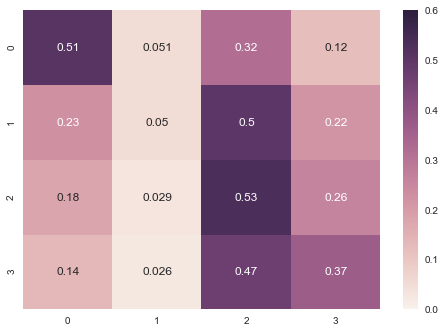
\includegraphics[width=0.7\textwidth]{heatmap_noclick.png}
  \caption{Heatmap that has no click data}
  \end{minipage}
  \begin{minipage}[t]{0.5\linewidth}
  \centering
  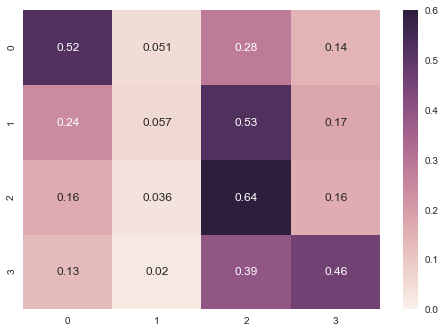
\includegraphics[width=0.7\textwidth]{heatmap_hasclick.png}
  \caption{Heatmap that has click data}
  \end{minipage}
\end{figure}


\section{Conclusion}
\label{conclusion}
In this project, we applied XGBoost to stock market by adding features of investor attention such as click numbers and favorite percente by investors . By tuning the parameters of XGBoost, we find XXX works best. Click number serves as the main engine to provide effective explanatory power among those sentiment analysis features. Favorite percentage and other multi-collinear terms may do harm to the whole model. 
%Click number can also predict next day’s return although the explanatory power and accuracy are not as strong as in explaining the same day return.



\section{Description of Individual Effort}

\section*{References}
[1]O. Netzer, R. Feldman, J. Goldenberg, M. FreskoMine your own business: market-structure surveillance through text mining
Marketing Science, 31 (3) (2012), pp. 521-543

[2]YangYu, Wenjing Duan, Qing Cao The impact of social and conventional media on firm equity value: A sentiment analysis approach 
Decision Support Systems Volume 55, Issue 4, November 2013, pp. 919-926

[3]Li, Tianyu Ray, et al. "Sentiment-based prediction of alternative cryptocurrency price fluctuations using gradient boosting tree model." arXiv preprint arXiv:1805.00558 (2018). 

[4]R. Gencay, Linear, non-linear and essential foreign ex-
change rate prediction with simple technical trading rules,
Journal of International Economics, vol. 47,no., pp. 91-107.19

[5]Bao D., Yang Z. (2008). Intelligent stock trading system by turning point confirming and probabilistic reasoning, Expert Systems with Applications, 34 (1), 620-627.

[6]Timmermann, A., Granger, C. W. (2004). Efficient market hypothesis and forecasting. Interational Journal of Forecasting. 20 (1), 15-27 

[7]Dey, Shubharthi, et al. Forecasting to Classification: Predicting the direction of stock market price using Xtreme Gradient Boosting. Working paper. DOI: 10.13140/RG. 2.2. 15294.48968.

[8]Yao, Juan, Chuanchan Ma, and William Peng He. "Investor herding behaviour of Chinese stock market." International Review of Economics \& Finance 29 (2014): 12-29.

[9]Qiu, Mingyue, and Yu Song. "Predicting the direction of stock market index movement using an optimized artificial neural network model." PloS one 11.5 (2016): e0155133.

[10]Chen T, Guestrin C. XGboost: A scalable tree boosting system. In Proceedings of the 22nd ACM SIG KDD International conference on Knowledge Discovery and Data Mining 2016 Aug 13 (pp. 785-794). ACM

\end{document}
